\documentclass[11pt,a4paper]{article}
\usepackage[utf8]{inputenc}
\usepackage[spanish,es-tabla]{babel}
\usepackage{amsmath}
\usepackage{amsfonts}
\usepackage{amssymb}
\usepackage{graphicx}
\usepackage{natbib}
\usepackage{lineno}
\usepackage{ragged2e}
\usepackage{multicol}
\setlength\columnsep{38pt}
\usepackage{enumerate} 
\usepackage[left=2.8cm,top=2.3cm,right=2.8cm,bottom=2.3cm]{geometry} 
\usepackage{fancyhdr}
\usepackage{url}
\usepackage{float}


\begin{document}
	
	\begin{center}
		\huge \textbf{Modelo Dimensional vs Modelo Tabular} 
	\end{center}
	\vspace{\baselineskip}
	\begin{center}
		
\includegraphics[scale=0.37]{./Imagenes/logo}
	\end{center}
	\vspace{\baselineskip}
	\begin{multicols}{2}
		\small
		\begin{center}
			Nelia Escalante Marón\\
			2014049551\\
			UPT – Ingeniería de Sistemas\\
			EPIS\\
			Tacna, Perú\\
			\vspace{\baselineskip}
			Yerson Coaquira Calizaya\\
			2015053225\\
			UPT – Ingeniería de Sistemas\\  
			EPIS\\
			Tacna, Perú\\                 
			\vspace{\baselineskip}
			Flor Condori Gutierrez\\
			2015053227\\
			UPT – Ingeniería de Sistemas\\  
			EPIS\\	
			Tacna, Perú\\                 
			\columnbreak
			
			\vspace{\baselineskip}
			Christian Cespedes Medina\\
			2010036256\\
			UPT – Ingeniería de Sistemas\\  
			EPIS\\	
			Tacna, Perú\\                 
			
			\vspace{\baselineskip}
			Javier Octavio Arteaga Ramos \\
			2007028981\\
			UPT – Ingeniería de Sistemas\\  
			EPIS\\	
			Tacna, Perú\\                 
			
		\end{center}
		\normalsize			
	\end{multicols}
	\vspace{\baselineskip}
	\vspace{\baselineskip}
	\vspace{\baselineskip}
	
	\textbf{\textit{\large Resumen}}\rule[1.5mm]{5mm}{0.1mm}		
	Desde el siglo pasado se ha investigado en aras de incrementar la eficiencia en el almacenamiento y el acceso a las bases de datos analíticas, sobre cuyos resultados las grandes compañías han introducido productos comerciales. En este escenario, Microsoft SQL Server 2012 ofrece dos opciones independientes para la creación de los modelos analíticos, el modelo multidimensional y el reciente modelo tabular. En este informe se profundiza en las características y potencialidades de cada uno, proponiendo los criterios más importantes que, a juicio de los autores, se deben tener en cuenta al emprender un nuevo proyecto. Se propone además una solución computacional que brinda a los especialistas y ejecutivos tanto visiones particulares como integradoras del estado del negocio, aprovechándose las facilidades recientes que proporciona la plataforma de Inteligencia de Negocios de Microsoft para la implementación de ambos modelos, dimensional y tabular.\\
	
	
	\newpage
	
	\textbf{\textit{\large Abstract}}\rule[1.5mm]{5mm}{0.1mm} 		
	\textit{
		Since the last century, research has been carried out in order to increase efficiency in storage and access to analytical databases, on the results of which large companies have introduced commercial products. In this scenario, Microsoft SQL Server 2012 offers two independent options for the creation of analytical models, the multidimensional model and the recent tabular model. This report delves into the characteristics and potential of each one, proposing the most important criteria that, in the opinion of the authors, should be taken into account when undertaking a new project. It is also proposed a computational solution that provides specialists and executives with both particular views and integrating the state of the business, taking advantage of the recent facilities provided by the Microsoft Business Intelligence platform for the implementation of both dimensional and tabular models.
	}
	
	\vspace{\baselineskip}
	
	\textbf{\textit{\large Keybwords}}\rule[1.5mm]{5mm}{0.1mm} 
	Modelos, Inteligencia de Negocios, Dimensional, Tabular.
	
	
	\rule{167mm}{0.1mm}
	
	\vspace{\baselineskip}
	
	 \section{INTRODUCCION}
	 
	 El siguiente trabajo fue hecho en consecuencia de un trabajo encargado para el curso de Inteligencia de Negocios.\\
	 \\
	 Consta de 2 partes: EL marco teórico y las referencias, la investigacion se ha hecho para la comparativa de dos tipos de modelados de tablas de base de datos en base a SQL: Modelado Dimensional y el Modelado Tabular.\\
	 \\
	 Unas de las principales caracteristicas que distiguen al modelo Tabular es que a nivel de consultas es muchisimo más veloz, como tambien que no necesita generar Agregaciones lo que simplifica el tiempo de procesamiento.\\
	 \\
	 En caso del modelo Dimensional su uso es necesario en caso que se quiera "jerarquizar" las tablas de un base de datos. En lo que destaca este modelo es su modo óptimo de organizar datos en los sistemas de Bussiness Intelligence  y lo mas destacable es que lo puede hacer mediante base de datos relacionales (ROLAP) o Base de Datos Dimensional (MOLAP). Se representa graficamente creando "estrellas" o "cubos".
	 	 
	 \section{MARCO TEÓRICO}
	 
	 	\subsection{Modelo Tabular}
	 	
	 	Los modelos tabulares son bases de datos “en memoria” de Analysis Services. Gracias a los algoritmos de compresión avanzados y al procesador de consultas multiproceso, el motor analítico en memoria xVelocity (VertiPaq) ofrece un acceso rápido a los objetos y los datos de los modelos tabulares para aplicaciones cliente de reportes como Microsoft Excel y Microsoft Power View.\\
	 	\\
	 	Los modelos tabulares admiten el acceso a los datos mediante dos modos: modo de almacenamiento en caché y modo DirectQuery. En el modo de almacenamiento en caché, puede integrar datos de varios orígenes como bases de datos relacionales, fuentes de distribución de datos y archivos de texto planos. En el modo DirectQuery, puede omitir el modelo en memoria, lo que permite a las aplicaciones cliente consultar los datos directamente en el origen relacional (SQL Server).
	 	Analysis Services proporciona funciones de procesamiento analítico en línea (OLAP) y minería de datos para aplicaciones de Business Intelligence.\\
	 	\\
	 		Los proyectos multidimensionales si bien les falta mucho para poder ser tan estables como las bases de datos transaccionales están en una etapa más avanzada de desarrollo y grandes empresas ya lo utilizan.[\cite{sanchez2015modelacion}]
	 	
	 	\begin{figure}[!ht]
	 		\begin{center}
	 			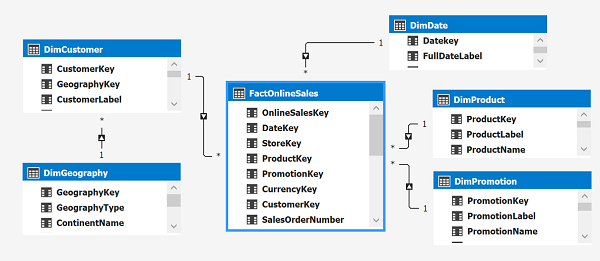
\includegraphics[scale=1.5]{./Imagenes/img01}	
	 			\caption{Modelo Tabular en SQL Server}		
	 		\end{center}
	 	\end{figure}
	 	
	 	\subsubsection{Ventajas del Modelo Tabular} 
	 	\begin{itemize}
	 		
	 		\item Mucho más veloz en consultas.
	 		\item No requiere generar Aggregations (agregaciones) por lo que se simplifica el tiempo de procesamiento.
	 		\item Gracias al DAX (el lenguaje para acceder a los datos equivalente al MDX), tiene mayor flexibilidad para obtener información.
	 		\item Es intuitivo por lo que es mucho más rápido y fácil de entender e implementar.
	 		\item Se basa en modelos relacionales.
	 		
	 	\end{itemize}
	 	
	 	\subsubsection{Problemas del Modelo Tabular} 
	 	\begin{itemize}
	 		
	 		\item Las particiones no se procesaban en paralelo si no secuencialmente, lo que hace que sea más lento el procesamiento.
	 		\item No se pueden usar múltiples idiomas.
	 		\item Si son muchos datos tarda bastante en manejar configuraciones de diferentes particiones.
	 		\item El modelo tabular acapara demasiada memoria RAM y a su vez es dependiente de tal que afectará a otras aplicaciones
	 		
	 	\end{itemize} 	
	 	
	 	\subsubsection{Sugerencias} 
	 	\begin{itemize}
	 		
	 		\item Primeramente, si ya se tiene una base de datos multidimensional, no se recomienda moverse a base de datos tabulares.
	 		\item El hardware requerido para un proyecto tabular es muy diferente al requerido por un proyecto multidimensional. Por la compresión de datos, requiere menos disco una modelo tabular, pero requiere mucha más memoria RAM porque todo lo usa en memoria. En general, se necesita un buen CPU y memoria.
	 		\item  Los modelos tabulares consumen muchos recursos, por lo que se recomienda hacer pruebas del funcionamiento en un servidor de desarrollo y no en producción.
	 		\item Se puede tener un modelo tabular y uno multidimensional instalados en la misma máquina, pero no es recomendable hacerlo en producción.
	 		
	 	\end{itemize} 
	 	
	 	\subsubsection{Jerarquías}
	 	Las jerarquías, en los modelos tabulares, son metadatos que definen las relaciones entre dos o más columnas de una tabla. Las jerarquías facilitan la navegación de los usuarios del cliente y su inclusión en un informe. 			
	 	\begin{figure}[H]
	 		\begin{center}
	 			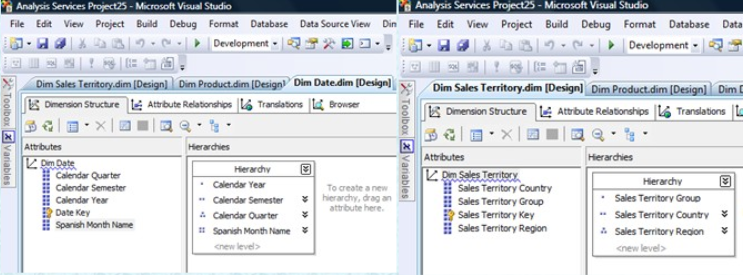
\includegraphics[scale=0.75]{./Imagenes/img02}	
	 			\caption{Jerarquías en el Modelo Tabular}		
	 		\end{center}
	 	\end{figure}
	 	
	 	Es una colección de niveles basados en atributos. Por ejemplo, una jerarquía de tiempo puede contener los niveles año, trimestre, mes, semana y día (ver imagen). Los usuarios finales pueden utilizar una jerarquía para examinar los datos del cubo. Se pueden revisar las propiedades de la Jerarquía con el menú contextual.			
	 	\begin{figure}[H]
	 		\begin{center}
	 			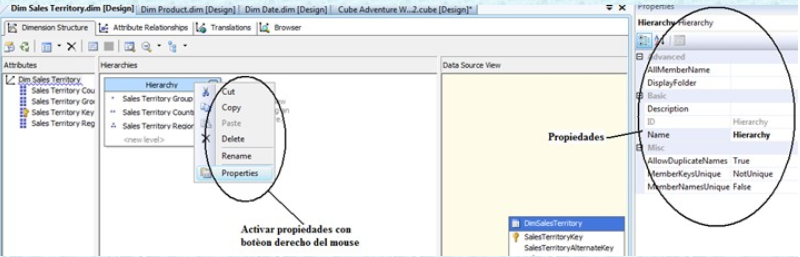
\includegraphics[scale=0.75]{./Imagenes/img03}	
	 			\caption{Método para mostrar las propiedades}	
	 		\end{center}
	 	\end{figure}
	 	\newpage
			\subsubsection{Tablas y relaciones en el modelo tabular en Power Bi}
			
			Cuando estamos desarrollando un proyecto de Business Intelligence con Power BI el punto fuerte de nuestro trabajo es garantizar que el modelo de datos esté debidamente diseñado para que funcione correctamente. Hay que mirar las tablas del modelo y comprobar la correcta definición de las relaciones entre ellas.
			Todo el tiempo que dediques a comprobar todas y cada una de las relaciones jugará a tu favor a la hora de crear las visualizaciones y los informes analíticos de tu proyecto de BI. Fíjate en la posición de cada tabla, en el lado que ocupan de la relación, Uno vs Muchos, en las columnas que intentas utilizar y si falla, comprueba que es la columna adecuada y que tiene el tipo adecuado.[\cite{cuevas2016comparing}]
			
			\begin{enumerate}[A.]
				\item Si la tabla está del lado Uno de la relación, todos los valores de la columna que utilizas son distintos y no hay nulos.
				\item Una vez que estés en la fase de visualización si obtienes resultados inesperados, como que el dato no se segmenta para cada filtro o que tienes valores nulos que no deben existir, regresa a comprobar la calidad de las relaciones definidas en tu modelo tabular. Por lo general allí encontrarás el problema y podrás darle solución.
				\item Hay dos aspectos que se admiten en la definición del modelo, las relaciones\textbf{ Muchos a Muchos} y la Dirección de filtro cruzado. No te lo recomiendo, puede ser muy problemático, a menos que ya seas un experto y estés muy seguro de todas las implicaciones de utilizar este tipo de configuración.
				\item No te compliques, no le hagas a Power BI más difícil el trabajo. Casi siempre, por no ser absoluta, es posible evitarlo. El modelo tabular es suficientemente rico y flexible como para permitirnos dar solución a los escenarios más complejos.  Y si no queda otra, hay que informarse muy bien de los posibles inconvenientes de este tipo de diseño.	
				\item Un elemento interesante es que si el modelo es complejo, podemos crear esquemas que segmenten la complejidad y muestren partes del modelo, lo que es bastante más cómodo de trabajar.
				
			\end{enumerate}
			
		\subsection{Modelo Dimensional}
		
		Hay un amplio acuerdo entre los usuarios de DataWarehouse de que el modelamiento dimensional es la mejor forma de presentar la información, porque es la mejor manera de reunir las principales metas de diseño:
			
			\begin{itemize}
				\item Presentar la información a los usuarios en la forma más simple posible.
				\item Retornar los resultados a los usuarios lo más rápido posible.
				\item Proveer información relevante que guarde pistas de los procesos subyacentes.
			\end{itemize}

		El modelo dimensional es mucho más fácil de entender para los usuarios que un sistema basado en un modelo normalizado de un sistema fuente típico, aunque un modelo dimensional típicamente contiene exactamente la misma información que un modelo normalizado.\\
		\\
		Un modelo dimensional tiene menos tablas y la información es agrupada en categorías de negocio coherentes que tienen sentido para los usuarios. Estas categorías ayudan a los usuarios a navegar por el modelo ya que categorías enteras pueden ser pasadas por alto si no son útiles para un determinado análisis\\
		\\
		\textit{\textbf{Según (Musso, 2012)}}, el Modelo Dimensional es una técnica de diseño lógico que tiene como objetivo presentar los datos dentro de un marco de trabajo estándar e intuitivo, para permitir su acceso con un alto rendimiento.\\
		\\
		\textit{\textbf{Según (Musso, 2012)}}, cada Modelo Dimensional está compuesto por una tabla con una llave combinada, llamada tabla de hechos, y con un conjunto de tablas más pequeñas llamadas tablas de dimensiones, como se muestra en la Figura 2. Los elementos de estas tablas se pueden definir de la siguiente manera:		
			\begin{itemize}
				\item \textbf{ Hechos:} es una colección de piezas de datos y datos de contexto. Cada hecho representa una parte del negocio, una transacción o un evento.
				\item \textbf{Dimensiones:} es una colección de miembros, unidades o individuos del mismo tipo.
				\item \textbf{Medidas:} son atributos numéricos de un hecho que representan el comportamiento del negocio relativo a una dimensión.
			\end{itemize}
		
			\begin{figure}[H]
				\begin{center}
					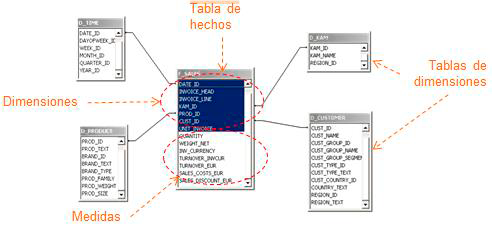
\includegraphics[scale=1.15]{./Imagenes/img05}	
					\caption{Deficion del modelo Dimensional}		
				\end{center}
			\end{figure}
		Cada punto de entrada a la tabla de hechos está conectado a una dimensión, lo que permite determinar el contexto de los hechos.\\
		\\
		\textit{\textbf{Por lo que (Musso, 2012)}} señala que dado que es muy común representar a un modelo dimensional como una tabla de hechos rodeada por las tablas de dimensiones, frecuentemente se le denomina también modelo estrella o esquema de estrella-unión. 
		
	 
	\bibliographystyle{apalike}
	\bibliography{BIBLIO}
	
	
\end{document}